\chapter{Miscellaneous and conclusions}
\minitoc
\emph{This final chapter will cover some additional configuration related to the MySQL database of Sguil. Next, some general facts are given non-related to Snort nor to Sguil. Finally, a general conclusion is formulated.}

\section{Sguil database optimization}

As Sguil is using a MySQL database to store its alerts, we can easily search for recommendations for optimizing this database by running the ``sudo mysqltuner'' command.

After the tuner has performed its job, the recommendations can be implemented by modifying the ``/etc/mysql/my.cnf'' file.

\begin{figure}[h]
    \centering
    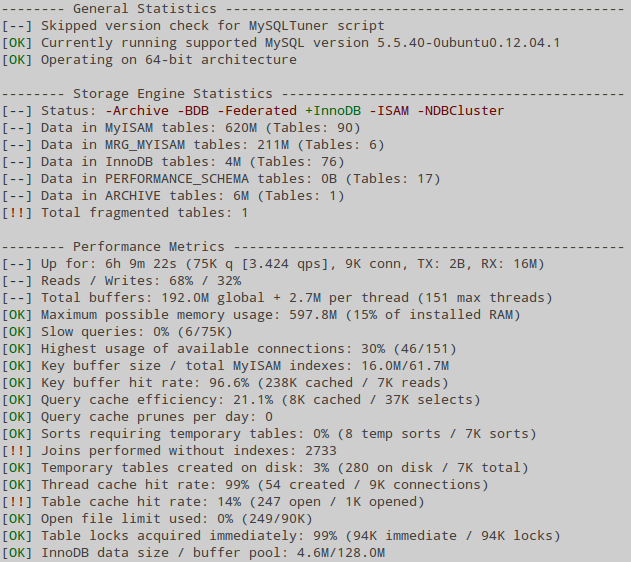
\includegraphics[width=0.85\textwidth]{VM_DB_11.png}
    \caption{Result of running the MySQL Tuner script.}
\end{figure}
\clearpage
\begin{figure}[h]
    \centering
    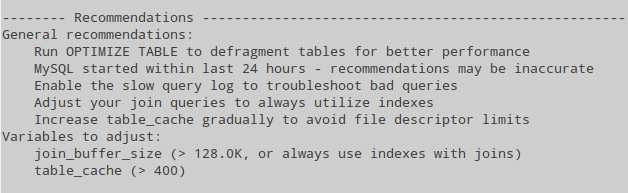
\includegraphics{VM_DB_12.png}
    \caption{Recommendations for optimizing the performance.}
\end{figure}
Here, the table cache (the number of files (tables) MySQL keeps open) is increased from 64 to 512.
\begin{figure}[h]
    \centering
    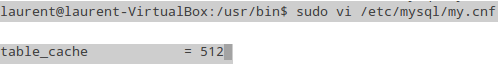
\includegraphics{VM_DB_13.png}
    \caption{The table\_cache is increased from 64 to 512}
\end{figure}
Of course, there exist many more options in this file that can be adjusted. Obviously, more possibilities to increase the performance of MySQL exist, but they will not be covered here since this is beyond the scope of this paper.
\clearpage

\section{General additional information}

In the screenshots below, the network traffic is displayed for the sniffing / capturing interface of Security Onion, being eth1. One can see that some day, this interface captured 1,2GB of packets circulating on the network. This was the day that the DOS attacks were performed.
\begin{figure}[h]
    \centering
    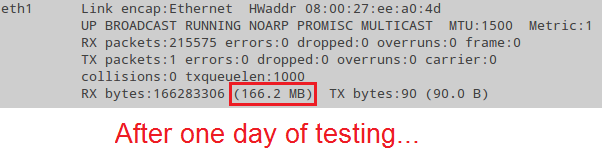
\includegraphics{VM_eth1.png}
    \caption{An ordinary day without DOS attacks\ldots}
\end{figure}

\begin{figure}[h]
    \centering
    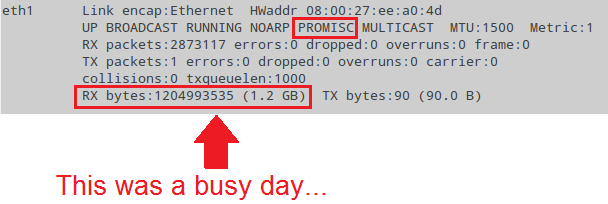
\includegraphics{VM_eth1_2.png}
    \caption{\ldots and a day that one of our machines was DOS'ed.}
\end{figure}
Below is a screenshot that gives the reader an idea of the system load of our physical machine running Security Onion. Also, one should make sure a decent CPU cooler is installed on the physical machine running Security Onion, as CPU load is almost always 100\%.
\begin{figure}[h]
    \centering
    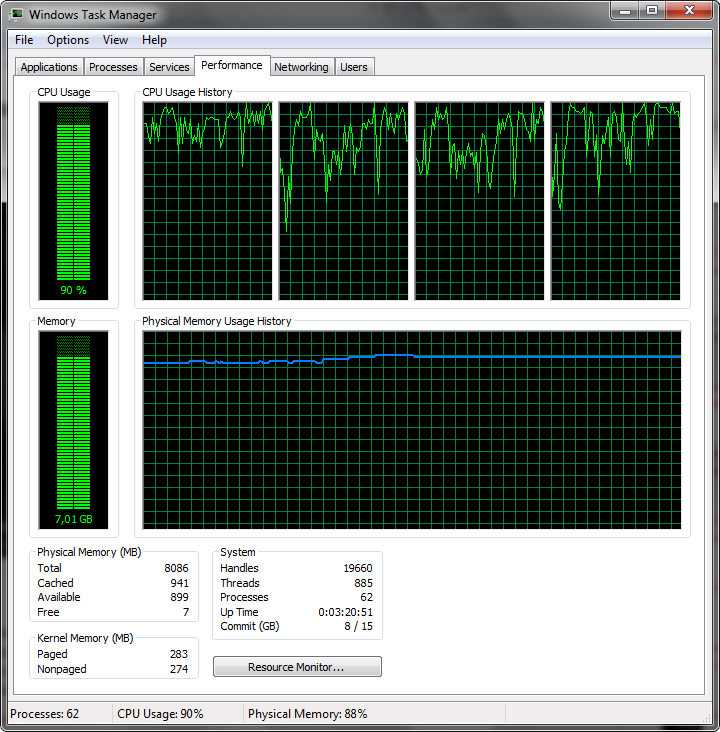
\includegraphics[width=0.55\textwidth]{VM_taskmanager_1.png}
    \caption{Security Onion is very demanding to the physical machine it is installed on.}
\end{figure}

\begin{figure}[h]
    \centering
    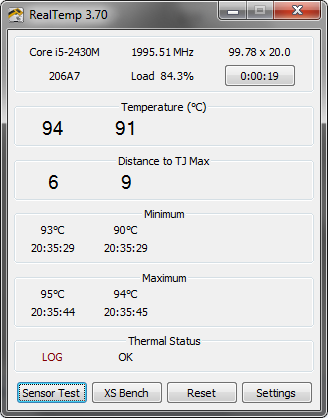
\includegraphics{VM_TEMP_1.png}
    \caption{Make sure you have a decent CPU cooler installed.}
\end{figure}
\clearpage
Finally, after the last day of testing and configuring Snort, we logged in into Snorby, the webapplication that provides a graphical overview of Snort events. The screenshots below provide an overview of the distribution of the Snort alerts.
\begin{figure}[h]
    \centering
    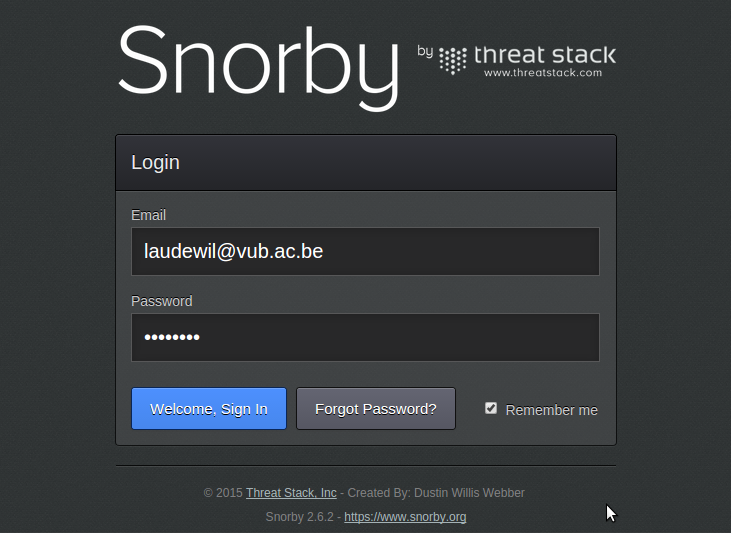
\includegraphics[width=0.65\textwidth]{VM_Snorby_1.png}
    \caption{The login screen of Snorby.}
\end{figure}
 \begin{figure}[h]
    \centering
    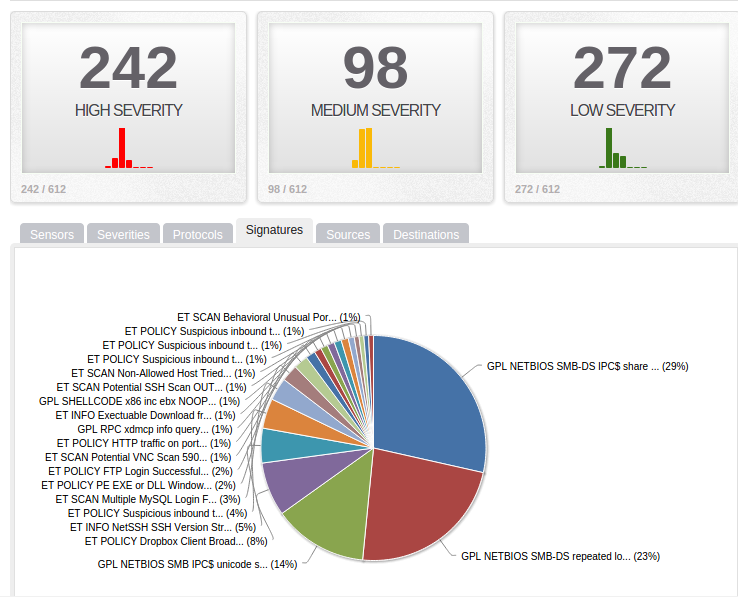
\includegraphics[width=0.65\textwidth]{VM_Snorby_4.png}
    \caption{The distribution of Snort alerts in percent.}
\end{figure}

\clearpage

\section{Conclusions}

After an intensive week of testing and configuring Snort, a general conclusion can be formulated: out-of-the-box, Snort performs relatively well, but in order to make Snort a  fully viable IDS on your specific network, additional configuration is required. \\ \\
Each network is different, so a general optimal configuration that is perfect for each network does not exist. Instead, one has to configure and fine-tune Snort to make in detect as much intrusions as possible and to minimize the amount of false positives. Obviously, this process takes up lots of time. \\ \\
This concludes the paper. 

